\documentclass[12pt,a4paper]{report}
\usepackage[utf8]{inputenc}
\usepackage[T5]{fontenc}
\usepackage[vietnamese]{babel}
\usepackage{graphicx}
\usepackage[hidelinks]{hyperref}
\usepackage{booktabs}
\usepackage{float}
\usepackage{geometry}
\usepackage{amsmath}
\usepackage{dirtytalk}
\geometry{a4paper, margin=1in}

\title{
    \vspace{2cm}
    \textbf{\Large BÁO CÁO MÔN TRÍ TUỆ NHÂN TẠO}\\
    \vspace{1cm}
    \textbf{\LARGE Xây dựng chatbot phân loại câu hỏi sử dụng thuật toán Naive Bayes}\\
    \vspace{2cm}
}

\author{
    \Large \textbf{Nhóm 11:}\\[0.5em]
    \large
    \begin{tabular}{l@{\hspace{1cm}}l}
        Nguyễn Quốc Việt & Mã SV: B25CHHT122 \\
        Uông Văn Công & Mã SV: B25CHHT080 \\
        Kim Anh Dũng & Mã SV: B25CHHT087 \\
    \end{tabular}\\[1.5cm]
    \Large \textbf{Giảng viên hướng dẫn:}\\[0.5em]
    \large TS. Đỗ Thanh Hà
}

\date{Ngày 18 tháng 4 năm 2026}

\begin{document}

\maketitle

\chapter*{Abstract}
\addcontentsline{toc}{chapter}{Abstract}
Báo cáo này trình bày quá trình nghiên cứu, thiết kế và phát triển một hệ thống chatbot hỗ trợ chẩn đoán bệnh dựa trên triệu chứng người dùng. Trong bối cảnh thông tin y tế trực tuyến thiếu kiểm chứng và dễ gây hoang mang, hệ thống hướng tới cung cấp công cụ nhận diện nguy cơ sức khỏe một cách nhanh chóng và đáng tin cậy nhờ ứng dụng trí tuệ nhân tạo. 

Mô hình sử dụng thuật toán Naive Bayes kết hợp với kỹ thuật TF-IDF để xử lý và biểu diễn dữ liệu văn bản. Nhằm khắc phục hạn chế về dữ liệu y tế tiếng Việt, nhóm đã áp dụng phương pháp sinh dữ liệu để xây dựng tập huấn luyện khoảng 20.000 câu hỏi đa dạng, gần với ngôn ngữ thực tế. 

Kết quả cho thấy hệ thống hoạt động ổn định, phản hồi nhanh và đạt độ chính xác khoảng 89\% trong phân loại 20 nhóm bệnh phổ biến.
\chapter*{Lời cảm ơn (Acknowledgements)}
\addcontentsline{toc}{chapter}{Lời cảm ơn}
Chúng em xin gửi lời cảm ơn chân thành đến TS. Đỗ Thanh Hà đã tận tâm hướng dẫn, cung cấp các nền tảng lý thuyết vững chắc về Trí tuệ Nhân tạo và tạo mọi điều kiện thuận lợi nhất để nhóm có thể hoàn thiện đồ án này.

\tableofcontents

\chapter{Giới thiệu (Introduction)}
Trí tuệ nhân tạo (AI) ngày càng đóng vai trò quan trọng trong hỗ trợ chẩn đoán và chăm sóc sức khỏe. Nhờ xử lý ngôn ngữ tự nhiên (NLP), máy tính có thể hiểu và phân tích các mô tả triệu chứng từ ngôn ngữ giao tiếp hằng ngày. Dự án \say{Xây dựng chatbot phân loại câu hỏi sử dụng thuật toán Naive Bayes} tập trung ứng dụng học máy để phân loại văn bản y tế. Hệ thống sử dụng mô hình xác suất để phân tích triệu chứng và đưa ra nhận định nhanh về các nhóm bệnh phổ biến, góp phần hỗ trợ người dùng định hướng thăm khám kịp thời và giảm tải cho hệ thống y tế.

\section{Tổng quan về các khái niệm}
Dự án xoay quanh hai kỹ thuật chính:
\begin{itemize}
    \item \textbf{Naive Bayes:} Thuật toán phân loại dựa trên định lý Bayes, tính xác suất một câu hỏi thuộc về nhóm bệnh nào dựa trên các từ khóa triệu chứng xuất hiện trong đó.
    \item \textbf{TF-IDF:} Phương pháp biểu diễn văn bản thành vector số, giúp đánh giá mức độ quan trọng của từng từ trong câu hỏi so với toàn bộ tập dữ liệu.
\end{itemize}
Hai kỹ thuật này được kết hợp để xây dựng một mô hình phân loại nhẹ, nhanh và phù hợp với dữ liệu tiếng Việt.

\section{Ứng dụng trong thực tế}
Phương pháp phân loại văn bản bằng Naive Bayes được ứng dụng rộng rãi trong nhiều lĩnh vực: lọc thư rác (Spam Filtering), phân tích cảm xúc khách hàng (Sentiment Analysis), phân loại bài báo theo chủ đề, và đặc biệt là hỗ trợ chẩn đoán y tế sơ bộ từ mô tả triệu chứng. Chi tiết về các ứng dụng sẽ được trình bày ở Chương 3.

\section{Mục tiêu (Objective)}
Khi có các triệu chứng như ho, sốt, đau ngực, người bệnh thường bối rối không biết mình có nguy cơ mắc bệnh gì. Việc tra cứu trên internet thiếu kiểm chứng có thể dẫn đến hoang mang không cần thiết (Cyberchondria).

Mục tiêu của dự án: \textbf{Tiếp nhận mô tả triệu chứng bằng ngôn ngữ tự nhiên và tính toán xác suất (\%) khả năng mắc 20 loại bệnh phổ biến.}
Hệ thống được phát triển với các tiêu chí:
\begin{itemize}
    \item Phân loại văn bản y tế tiếng Việt (Text Classification).
    \item Xử lý nhanh, nhẹ nhờ thuật toán Naive Bayes.
    \item Giao diện web thân thiện, tối ưu cho thiết bị di động.
\end{itemize}

\section{Các nghiên cứu liên quan (Related works)}
\subsection{Cách tiếp cận truyền thống (Classical approaches)}
Các hệ thống tư vấn sức khỏe trước đây thường dùng luật if-else (Rule-based). Ưu điểm là dễ hiểu, dễ kiểm soát. Nhược điểm là cồng kềnh và khó xử lý được sự đa dạng trong cách diễn đạt của người dùng.

\subsection{Học sâu (Deep Learning)}
Các mô hình lớn như Transformer, BERT hiểu ngữ cảnh tốt nhưng đòi hỏi phần cứng mạnh và lượng dữ liệu lớn. Do hạn chế về tài nguyên và thời gian, nhóm chọn TF-IDF kết hợp Naive Bayes vì chạy nhẹ, huấn luyện nhanh và vẫn cho kết quả tốt trên dữ liệu nhỏ.

\chapter{Cơ sở lý thuyết (Fundamental concepts)}

\section{Xử lý ngôn ngữ tự nhiên (NLP)}
Xử lý ngôn ngữ tự nhiên (Natural Language Processing - NLP) là lĩnh vực nghiên cứu giúp máy tính hiểu và xử lý ngôn ngữ của con người. Trong dự án này, NLP đóng vai trò tiền xử lý dữ liệu đầu vào trước khi đưa vào mô hình phân loại.

Các bước tiền xử lý chính:
\begin{itemize}
    \item \textbf{Tách từ (Word Segmentation):} Tiếng Việt là ngôn ngữ đơn lập, một từ có thể gồm nhiều âm tiết (ví dụ: \say{đau đầu}, \say{khó thở}). Hệ thống sử dụng thư viện \textbf{Underthesea} để tách từ tiếng Việt chính xác.
    \item \textbf{Chuyển chữ thường:} Đồng nhất \say{Sốt}, \say{sốt}, \say{SỐT} thành một dạng duy nhất.
    \item \textbf{Loại bỏ từ dừng (Stop words):} Loại các từ không mang ý nghĩa phân loại như \say{tôi}, \say{bị}, \say{rất}, \say{thì}... để giảm nhiễu cho mô hình.
\end{itemize}

\textbf{Ví dụ:} Câu nhập \textit{\say{Tôi bị đau đầu và sốt cao}} sau tiền xử lý sẽ thành: \texttt{đau\_đầu sốt cao}.

\section{Biểu diễn văn bản bằng TF-IDF}
Máy tính không thể xử lý trực tiếp trên chữ viết, do đó cần chuyển văn bản thành dạng vector số. TF-IDF (Term Frequency -- Inverse Document Frequency) là phương pháp được sử dụng trong dự án.

\subsection{TF -- Tần suất từ (Term Frequency)}
Đo số lần một từ xuất hiện trong một văn bản, chuẩn hóa theo tổng số từ:
\[ \text{TF}(t, d) = \frac{\text{Số lần từ } t \text{ xuất hiện trong văn bản } d}{\text{Tổng số từ trong văn bản } d} \]

\subsection{IDF -- Nghịch tần suất văn bản (Inverse Document Frequency)}
Đánh giá mức độ đặc biệt của một từ trong toàn bộ tập dữ liệu. Từ xuất hiện ở quá nhiều văn bản sẽ có IDF thấp:
\[ \text{IDF}(t) = \log \frac{N}{1 + \text{DF}(t)} \]
Trong đó $N$ là tổng số văn bản, $\text{DF}(t)$ là số văn bản chứa từ $t$.

\subsection{Kết hợp TF-IDF}
Trọng số cuối cùng của mỗi từ:
\[ \text{TF-IDF}(t, d) = \text{TF}(t, d) \times \text{IDF}(t) \]

\textbf{Ví dụ:} Từ \say{sốt} xuất hiện ở hầu hết các bệnh nên có IDF thấp. Ngược lại, từ \say{mắt\_vàng} chỉ xuất hiện ở bệnh viêm gan nên có IDF cao, giúp mô hình phân biệt tốt hơn.

\section{Định lý Bayes}
Định lý Bayes mô tả xác suất xảy ra của một sự kiện dựa trên các bằng chứng đã biết:
\[ P(C \,|\, X) = \frac{P(X \,|\, C) \cdot P(C)}{P(X)} \]

Giải thích từng thành phần trong bài toán chẩn đoán bệnh:
\begin{itemize}
    \item $P(C \,|\, X)$: Xác suất mắc bệnh $C$ khi đã biết triệu chứng $X$ (\textbf{posterior}).
    \item $P(X \,|\, C)$: Xác suất xuất hiện triệu chứng $X$ ở người mắc bệnh $C$ (\textbf{likelihood}).
    \item $P(C)$: Xác suất mắc bệnh $C$ trong tập dữ liệu (\textbf{prior}).
    \item $P(X)$: Xác suất xuất hiện triệu chứng $X$ nói chung (\textbf{evidence}).
\end{itemize}

\section{Thuật toán Multinomial Naive Bayes}
Naive Bayes có nhiều biến thể. Dự án sử dụng \textbf{Multinomial Naive Bayes} vì phù hợp với bài toán phân loại văn bản, nơi đặc trưng đầu vào là tần suất xuất hiện của các từ.

\subsection{Giả định ``Naive'' (Ngây thơ)}
Thuật toán giả định rằng các từ trong câu hỏi xuất hiện \textbf{độc lập} với nhau. Ví dụ: sự xuất hiện của từ \say{sốt} không ảnh hưởng đến xác suất xuất hiện của từ \say{ho}. Trong thực tế, giả định này không hoàn toàn đúng, nhưng mô hình vẫn cho kết quả phân loại tốt nhờ tính đơn giản và hiệu quả.

\subsection{Công thức phân loại}
Với một câu hỏi gồm các từ $x_1, x_2, ..., x_n$, lớp bệnh được dự đoán là:
\[ \hat{C} = \arg\max_{C} \; P(C) \prod_{i=1}^{n} P(x_i \,|\, C) \]

Để tránh tích xác suất quá nhỏ, trong thực tế ta dùng logarit:
\[ \hat{C} = \arg\max_{C} \left[ \log P(C) + \sum_{i=1}^{n} \log P(x_i \,|\, C) \right] \]

\subsection{Xử lý Laplace Smoothing}
Nếu một từ chưa từng xuất hiện trong dữ liệu huấn luyện của một lớp bệnh, $P(x_i \,|\, C) = 0$ sẽ làm toàn bộ tích bằng 0. Để khắc phục, áp dụng phép làm mượt Laplace với hệ số $\alpha = 1.0$:
\[ P(x_i \,|\, C) = \frac{\text{count}(x_i, C) + \alpha}{\sum_{j} \text{count}(x_j, C) + \alpha \cdot |V|} \]
Trong đó $|V|$ là kích thước bộ từ vựng.

\section{Pipeline phân loại tổng thể}
Toàn bộ quy trình xử lý từ đầu vào đến kết quả được mô tả qua các bước:
\begin{enumerate}
    \item \textbf{Nhập liệu:} Người dùng nhập mô tả triệu chứng bằng tiếng Việt.
    \item \textbf{Tiền xử lý NLP:} Tách từ (Underthesea), chuyển chữ thường, loại bỏ từ dừng.
    \item \textbf{Vector hóa TF-IDF:} Chuyển văn bản đã xử lý thành vector số.
    \item \textbf{Phân loại Naive Bayes:} Tính xác suất cho từng nhóm bệnh, chọn nhóm có xác suất cao nhất.
    \item \textbf{Trả kết quả:} Hiển thị tên bệnh kèm phần trăm xác suất dự đoán.
\end{enumerate}

\chapter{Ứng dụng (Applications)}
Thuật toán phân loại văn bản (Text Classification) và đặc biệt là Naive Bayes là một trong những giải pháp máy học nền tảng, được ứng dụng rộng rãi trong nhiều lĩnh vực thực tiễn.

\section{Ứng dụng trong Y tế và Chăm sóc sức khỏe}

\subsection{Hỗ trợ chẩn đoán bệnh từ triệu chứng}
Nhiều nền tảng y tế trực tuyến đã ứng dụng AI để hỗ trợ người dùng nhận diện nguy cơ sức khỏe. Các ứng dụng như \textbf{Ada Health}, \textbf{Symptomate} hay \textbf{WebMD Symptom Checker} cho phép người dùng mô tả triệu chứng và nhận về danh sách bệnh có khả năng mắc phải. Naive Bayes phù hợp cho bài toán này vì:
\begin{itemize}
    \item Tính toán nhanh, cho kết quả gần như tức thì.
    \item Hoạt động tốt ngay cả khi dữ liệu huấn luyện không quá lớn.
    \item Trả về xác suất cho từng nhóm bệnh, giúp người dùng đánh giá mức độ nguy cơ.
\end{itemize}

\subsection{Phân loại và sàng lọc hồ sơ y tế}
Trong các bệnh viện lớn, lượng hồ sơ bệnh án tích lũy qua nhiều năm là rất lớn. Thuật toán phân loại văn bản giúp tự động gán nhãn chuyên khoa cho hồ sơ (Nội khoa, Ngoại khoa, Da liễu...), hỗ trợ bác sĩ tra cứu nhanh các ca bệnh tương tự trong quá khứ.

\section{Ứng dụng trong Công nghệ thông tin}

\subsection{Lọc thư rác (Spam Filtering)}
Đây là một trong những ứng dụng kinh điển và thành công nhất của Naive Bayes. Hệ thống email \textbf{Gmail} từ những ngày đầu đã sử dụng bộ lọc dựa trên Bayesian Filter để phân biệt thư hợp lệ và thư rác. Nguyên lý hoạt động: dựa trên tần suất xuất hiện của các từ khóa đặc trưng (như \say{khuyến mãi}, \say{trúng thưởng}, \say{miễn phí}...), thuật toán tính xác suất email đó là spam. Ưu điểm là mô hình có thể \textbf{tự học và cập nhật} khi người dùng đánh dấu thư rác mới.

\subsection{Phân tích cảm xúc (Sentiment Analysis)}
Trong thương mại điện tử, các sàn như \textbf{Shopee}, \textbf{Tiki}, \textbf{Amazon} cần tự động phân loại hàng triệu bình luận đánh giá sản phẩm thành các nhóm: \say{Tích cực}, \say{Tiêu cực} hoặc \say{Trung lập}. Naive Bayes kết hợp TF-IDF là giải pháp baseline phổ biến vì:
\begin{itemize}
    \item Huấn luyện nhanh trên lượng dữ liệu lớn.
    \item Dễ triển khai và bảo trì trong môi trường production.
    \item Độ chính xác đủ tốt cho tác vụ phân loại 2--3 lớp.
\end{itemize}

\subsection{Phân loại tin tức và nội dung}
Các trang tin tức lớn như \textbf{VnExpress}, \textbf{Báo Mới} sử dụng thuật toán phân loại văn bản để tự động gán thẻ chuyên mục (Thể thao, Kinh doanh, Đời sống, Công nghệ...) cho bài viết mới. Naive Bayes nhận diện chuyên mục dựa trên phân bố từ vựng đặc trưng của từng lĩnh vực, ví dụ: bài chứa nhiều từ \say{bàn thắng}, \say{cầu thủ}, \say{giải đấu} sẽ được xếp vào mục Thể thao.

\section{Ứng dụng của dự án}
Dự án này áp dụng chính các kỹ thuật trên vào bài toán \textbf{chẩn đoán bệnh sơ bộ cho người Việt}. So với các hệ thống quốc tế (Ada Health, Symptomate), dự án tập trung vào:
\begin{itemize}
    \item Xử lý \textbf{tiếng Việt} với đặc thù tách từ đa âm tiết.
    \item Giao diện đơn giản dạng \textbf{chatbot}, phù hợp với thói quen sử dụng của người dùng phổ thông.
    \item Mô hình nhẹ, có thể chạy trên máy cá nhân mà không cần GPU hay hạ tầng phức tạp.
\end{itemize}

\section{Triển khai phần mềm và thực nghiệm}
\subsection{Kiến trúc hệ thống và Dữ liệu}
Hệ thống tuân thủ kiến trúc chia tách rạch ròi:
\begin{itemize}
    \item \textbf{Client (Frontend):} Thiết kế thuần HTML5/CSS3/ES6, giao diện dạng chatbot trực quan tối giản theo định hướng y tế.
    \item \textbf{Server (Backend):} Triển khai Web Server bằng module Flask trong Python.
    \item \textbf{Core (Machine Learning):} Scikit-Learn (MultinomialNB và TfidfVectorizer) kết hợp xử lý phân tách từ tiếng Việt tự nhiên bằng thư viện Underthesea.
\end{itemize}

Dữ liệu huấn luyện được sinh tự động thông qua việc trộn tổ hợp các triệu chứng cốt lõi của 20 nhóm bệnh với các tiền tố/hậu tố giao tiếp thông dụng. Quá trình sinh dữ liệu đã tạo ra khoảng 20.000 dòng dữ liệu văn bản đại diện, phong phú, giúp mô hình học tập tốt hơn. 

Dưới đây là một phần trích xuất nhỏ từ tập dữ liệu thực tế nhằm minh họa cách hệ thống tự động sinh câu và gán nhãn (Auto-labeling) trước khi đưa vào huấn luyện Classifier:

\begin{table}[H]
\centering
\begin{tabular}{|l|p{9.5cm}|}
\hline
\textbf{Nhãn bệnh (Disease Label)} & \textbf{Văn bản huấn luyện (Symptom Text)} \\ \hline
Sốt xuất huyết & Bác sĩ ơi tôi bị sốt cao liên tục, phát ban, nhức mỏi cơ \\ \hline
Đái tháo đường & Tự nhiên bị khát nước liên tục, sụt cân không nguyên nhân \\ \hline
Viêm phổi & Tôi bị đau ngực, ho dai dẳng, sốt lừ đừ \\ \hline
Viêm loét dạ dày & Mấy hôm nay tôi bị đau bụng thượng vị, ợ chua, buồn nôn \\ \hline
Sỏi thận & Cháu bị đau quặn thắt lưng, ớn lạnh, đi tiểu ra máu \\ \hline
\end{tabular}
\caption{Trích xuất 5 mẫu minh họa trong rổ 20.000 dòng dữ liệu huấn luyện}
\label{tab:data_sample}
\end{table}

\subsection{Kết quả thực nghiệm}
Sau quá trình huấn luyện trên máy cá nhân với bù trừ nhẵn Laplace $\alpha=1.0$, mô hình Naive Bayes đạt được tỷ lệ chính xác (Accuracy): \textbf{89.0\%} trên tập kiểm thử (16.000 dòng train, 4.000 dòng test).

Kết quả 10 testcase:

\begin{table}[H]
\centering
\begin{tabular}{|c|p{5.5cm}|l|p{4.5cm}|}
\hline
\textbf{\#} & \textbf{Câu chat gõ vào UI} & \textbf{Chẩn đoán AI} & \textbf{Đánh giá} \\ \hline
1 & Tôi bị sốt cao, ho dai dẳng & Viêm phổi & Nhận diện tốt cụm ``ho dai dẳng'' \\ \hline
2 & Bị hắt hơi sổ mũi, sốt nhẹ & Cảm cúm & Phân loại đúng bệnh lý thường gặp \\ \hline
3 & Phát ban, chảy máu chân răng & Sốt xuất huyết & Xác định tốt dấu hiệu đặc thù \\ \hline
4 & Ợ chua khó tiêu, đau vùng thượng vị & Viêm loét dạ dày & Nhận diện chính xác vùng tiêu hóa \\ \hline
5 & Ăn xong nôn mửa tiêu chảy & Ngộ độc thực phẩm & Chẩn đoán chính xác \\ \hline
6 & Tiểu rắt, đau quặn thắt lưng & Sỏi thận & Mức độ khớp đặc điểm cao \\ \hline
7 & Mắt vàng da vàng, mệt mỏi & Viêm gan & Dấu hiệu quá rõ ràng, AI dự đoán chuẩn \\ \hline
8 & Cứng khớp, lạo xạo đầu gối & Thoái hóa khớp & Lấy tốt được từ khóa chuyên khoa \\ \hline
9 & Hoa mắt, buồn nôn khi đứng & Rối loạn tiền đình & Xác suất phản ánh thực tế rất tốt \\ \hline
10 & Nổi mẩn ngứa sưng đỏ & Dị ứng da & Tách từ tiếng Việt hoạt động hiệu quả \\ \hline
\end{tabular}
\caption{Bảng 10 Kịch bản kiểm thử trực tiếp trên Web Chatbot}
\end{table}

\begin{figure}[H]
    \centering
    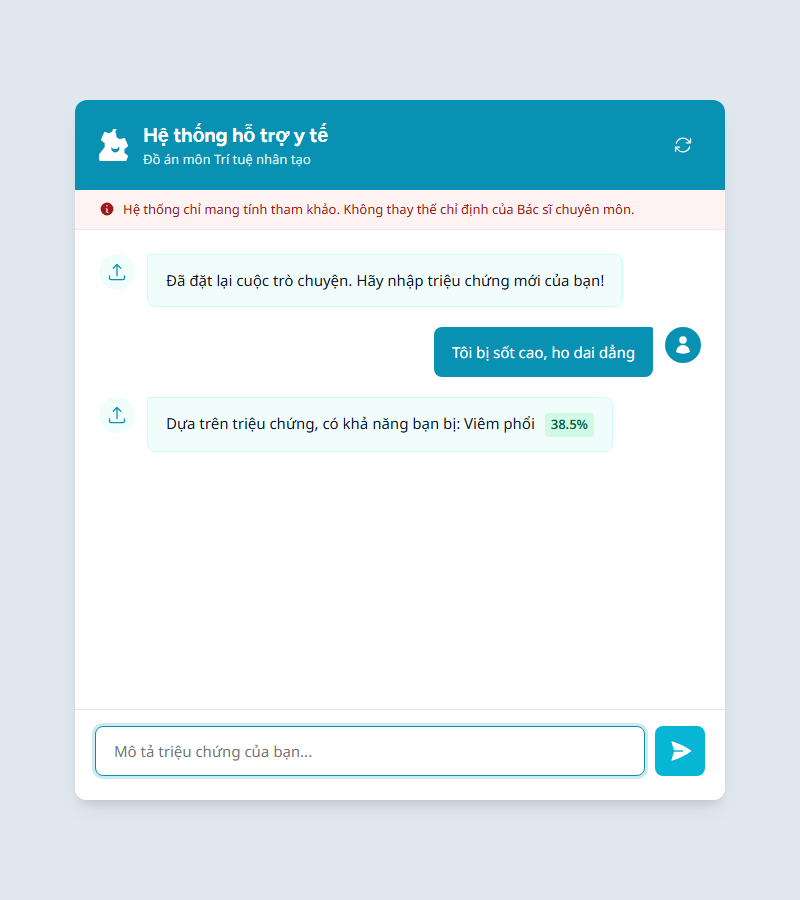
\includegraphics[width=0.8\textwidth]{images/test_1.png}
\end{figure}

\begin{figure}[H]
    \centering
    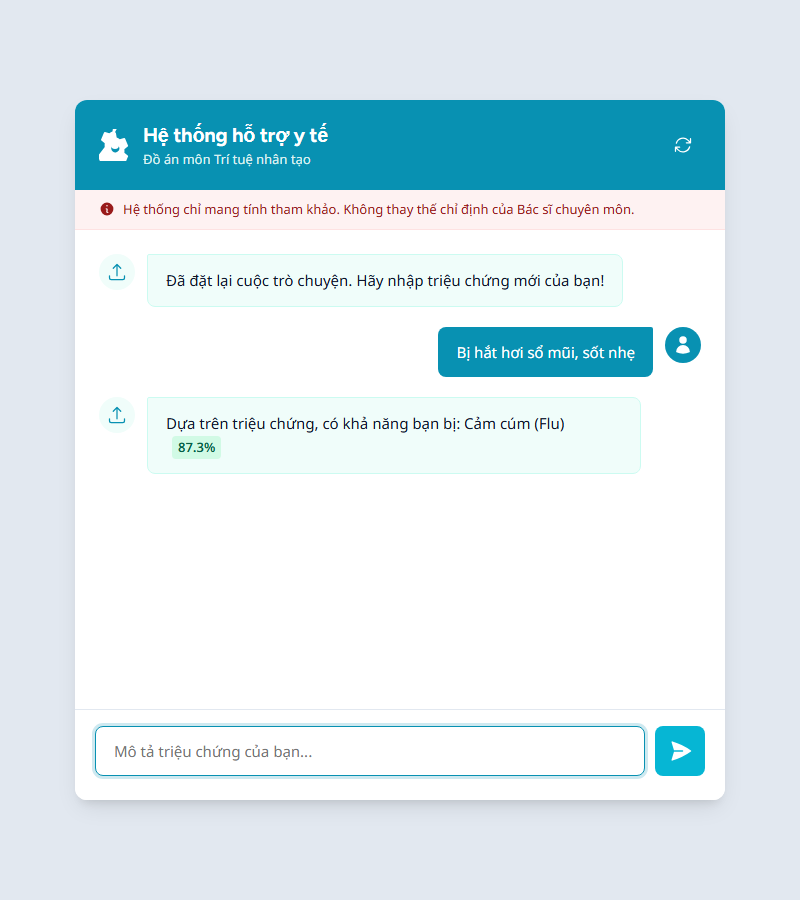
\includegraphics[width=0.8\textwidth]{images/test_2.png}
\end{figure}

\begin{figure}[H]
    \centering
    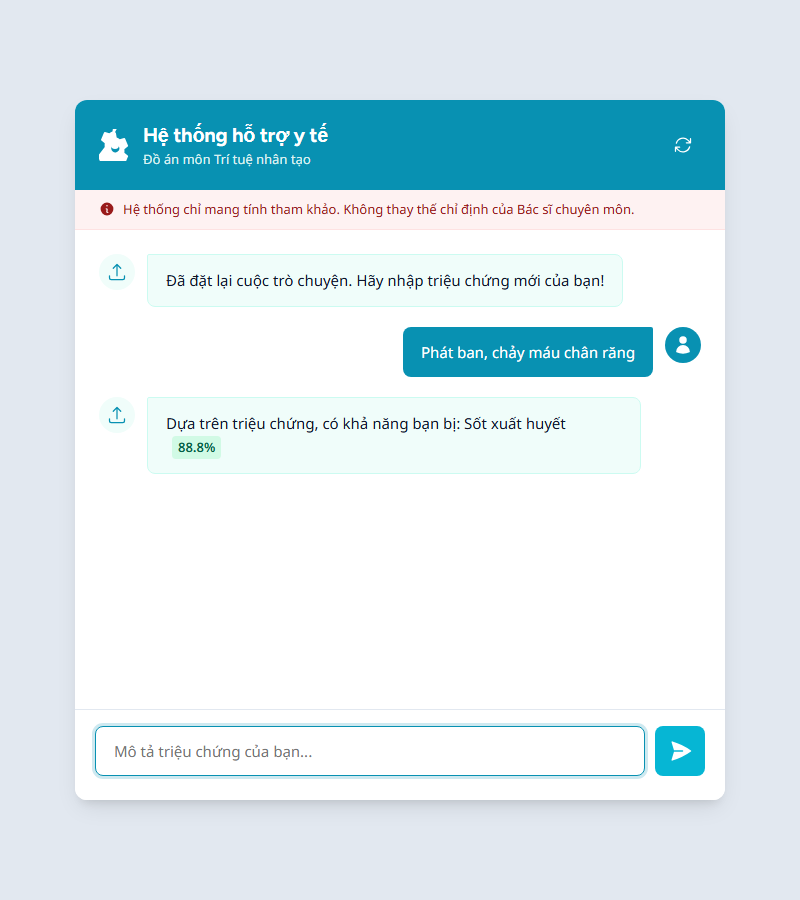
\includegraphics[width=0.8\textwidth]{images/test_3.png}
\end{figure}

\begin{figure}[H]
    \centering
    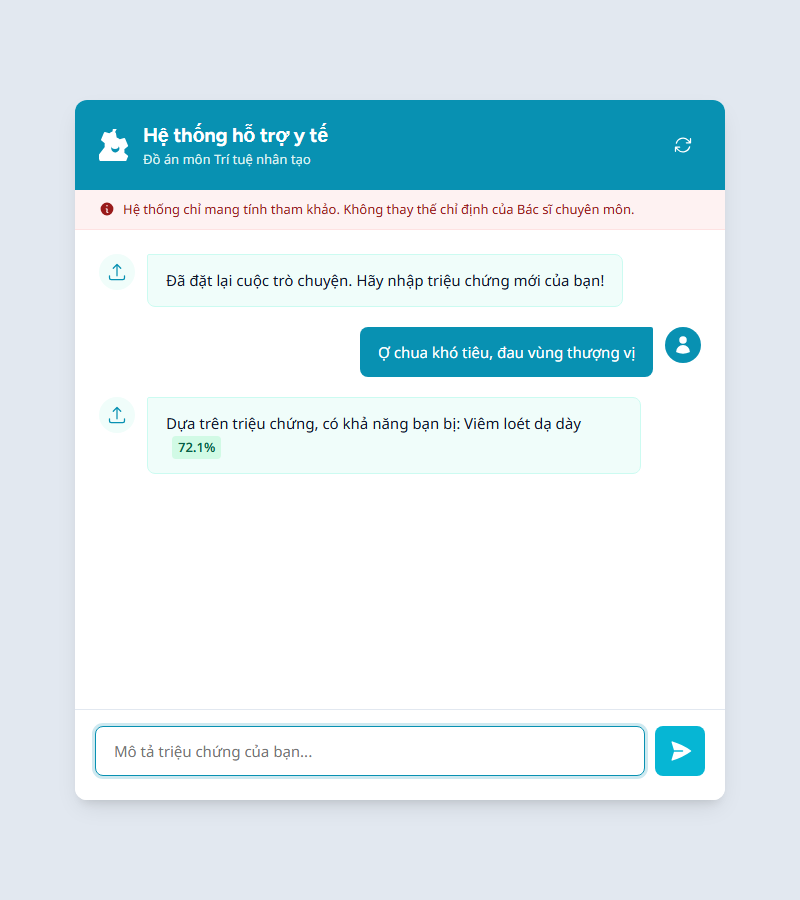
\includegraphics[width=0.8\textwidth]{images/test_4.png}
\end{figure}

\begin{figure}[H]
    \centering
    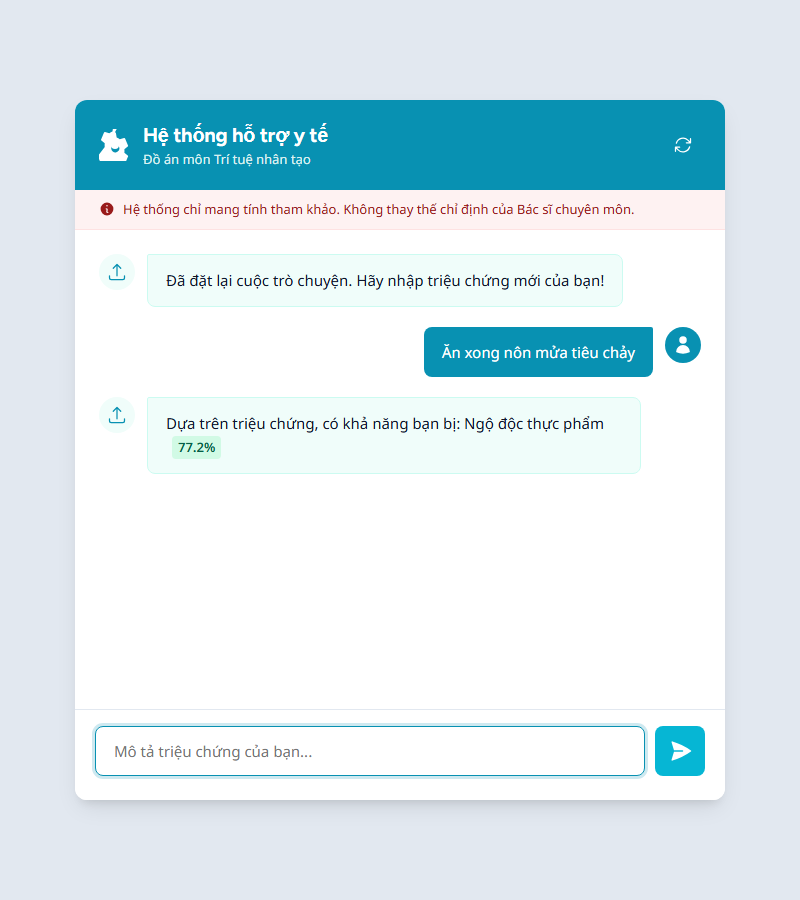
\includegraphics[width=0.8\textwidth]{images/test_5.png}
\end{figure}

\begin{figure}[H]
    \centering
    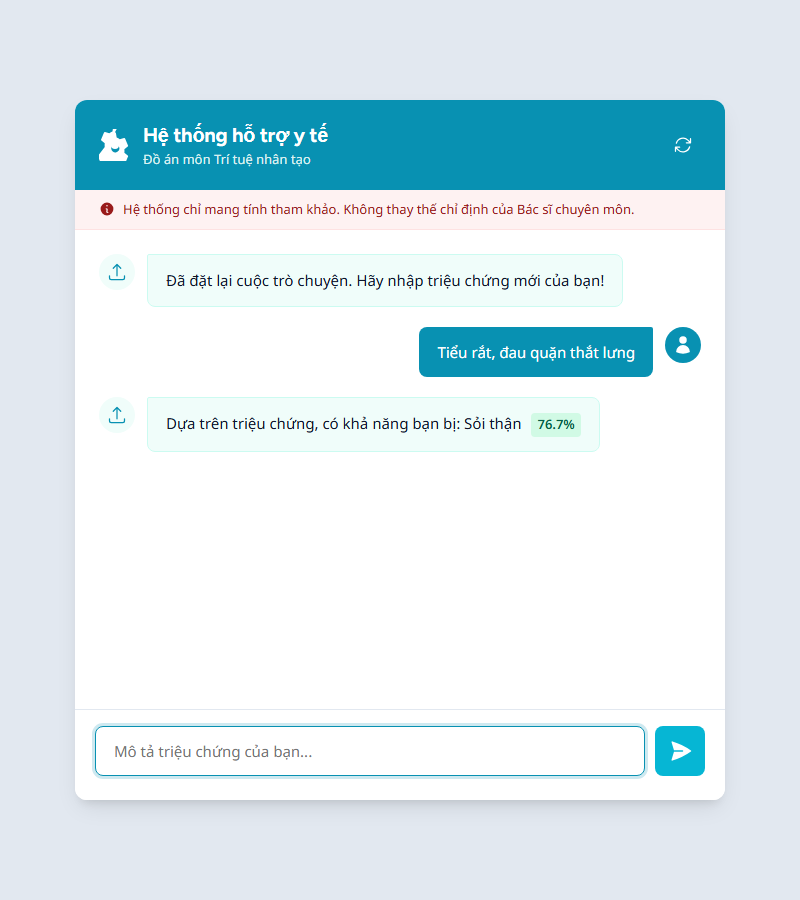
\includegraphics[width=0.8\textwidth]{images/test_6.png}
\end{figure}

\begin{figure}[H]
    \centering
    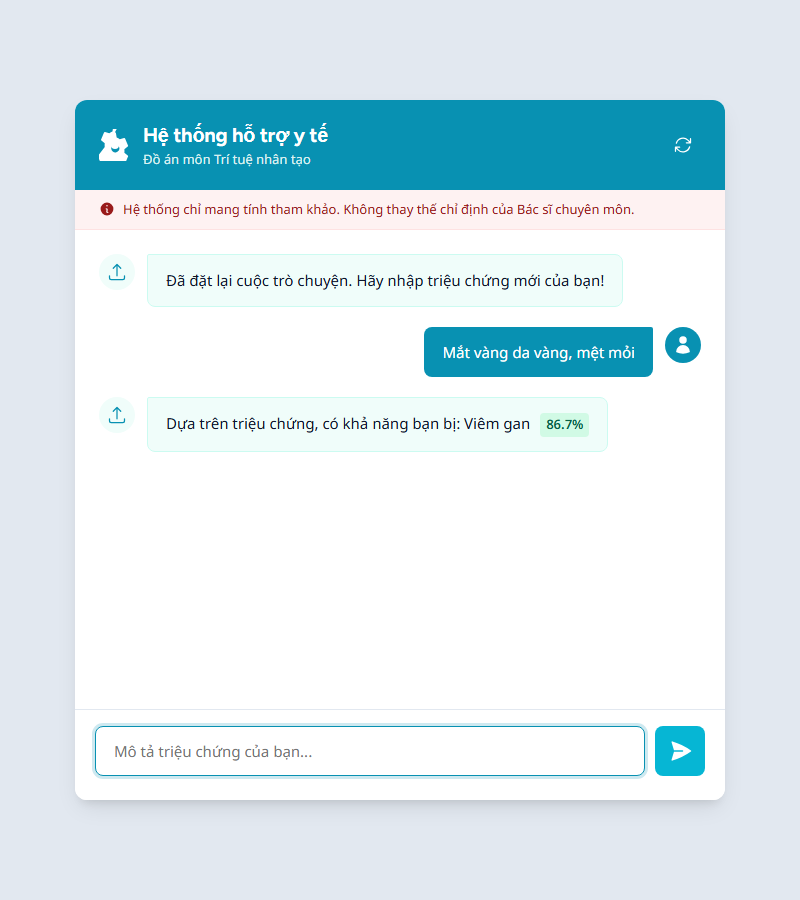
\includegraphics[width=0.8\textwidth]{images/test_7.png}
\end{figure}

\begin{figure}[H]
    \centering
    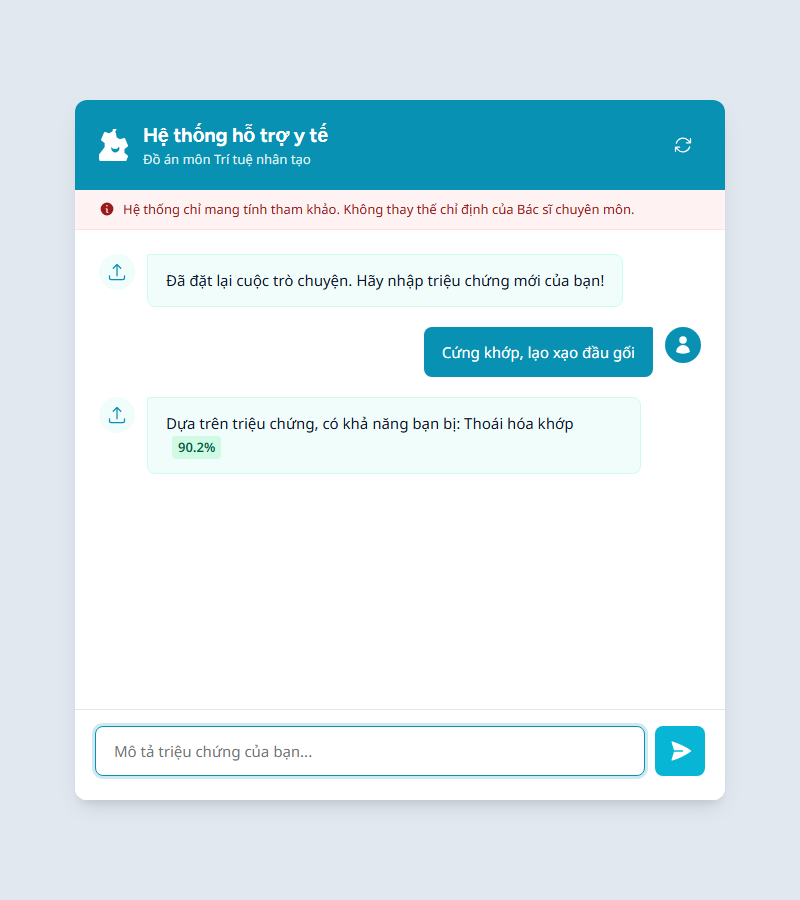
\includegraphics[width=0.8\textwidth]{images/test_8.png}
\end{figure}

\begin{figure}[H]
    \centering
    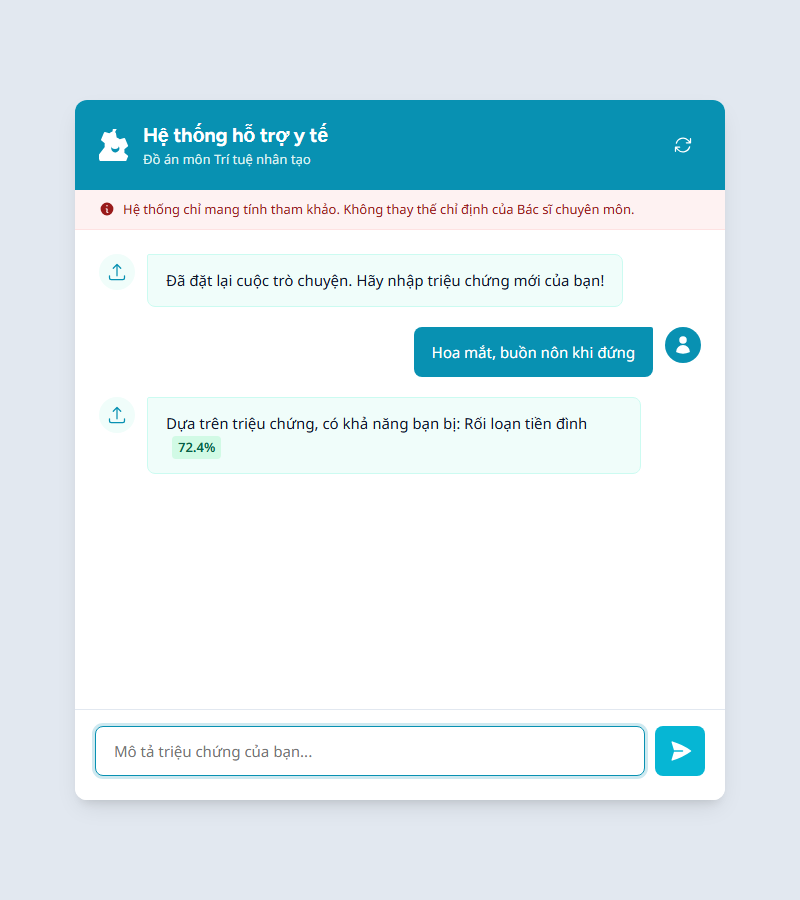
\includegraphics[width=0.8\textwidth]{images/test_9.png}
\end{figure}

\begin{figure}[H]
    \centering
    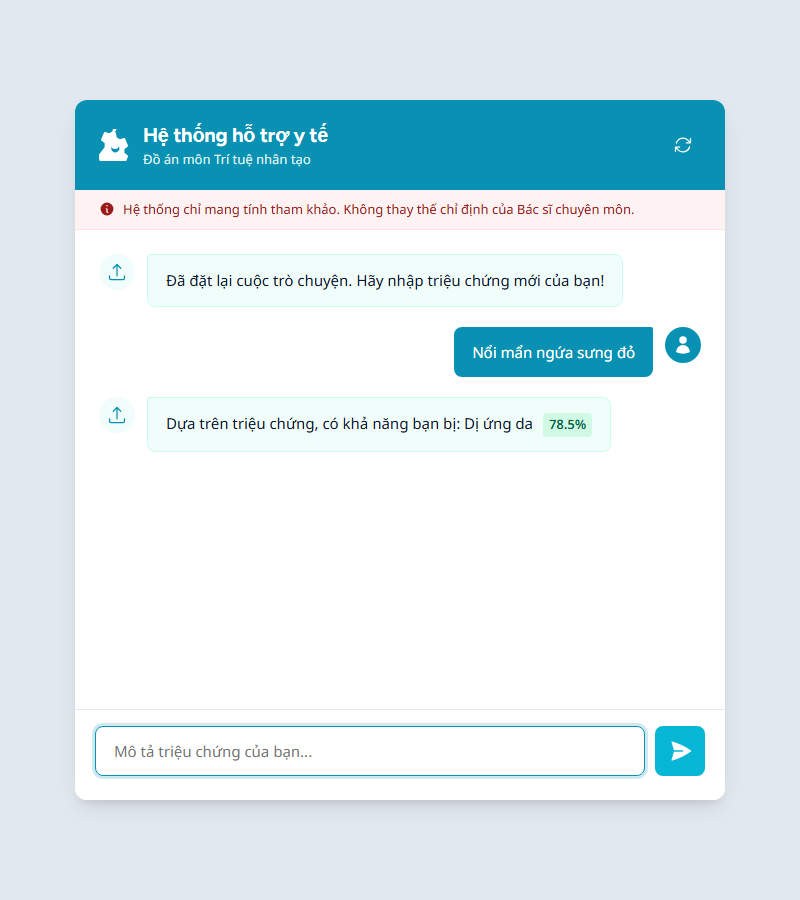
\includegraphics[width=0.8\textwidth]{images/test_10.png}
    \caption{Các giao diện kết quả kiểm thử 10 kịch bản trên ứng dụng}
    \label{fig:app_test}
\end{figure}

\addcontentsline{toc}{chapter}{Tài liệu tham khảo (References)}
\begin{thebibliography}{9}

\bibitem{scikit_learn} 
Scikit-learn developers, 2026. \textit{Naive Bayes}. [online] Available at: $<$https://scikit-learn.org/stable/modules/naive\_bayes.html$>$ [Accessed 18 April 2026].

\bibitem{underthesea}
Underthesea NLP Team, 2026. \textit{Vietnamese NLP Toolkit}. [online] Available at: $<$https://github.com/undertheseanlp/underthesea$>$ [Accessed 18 April 2026].

\end{thebibliography}

\end{document}
